Listing\section{Extraction Process: Index}
\label{sec:index}
%% - Welche Arten von Indexeinträgen gibt es? Wie ist ein einzelner
%%   Indexeintrag aufgebaut (jeweils für alle Typen)?
%% - XML-Schema für einzelne Indexeinträge beschreiben / erklären;
%%   jeweils mit (konstruiertem) Beispiel, in dem alles vorkommt
%% - Extraktion beschreiben (control flow, evtl. als Diagramm; Behandlung
%%   von Sonderfällen / Ausnahmen; etc.)

\emph{Author: Susanne Fertmann} \\

\begin{figure}[h]
  \centering
  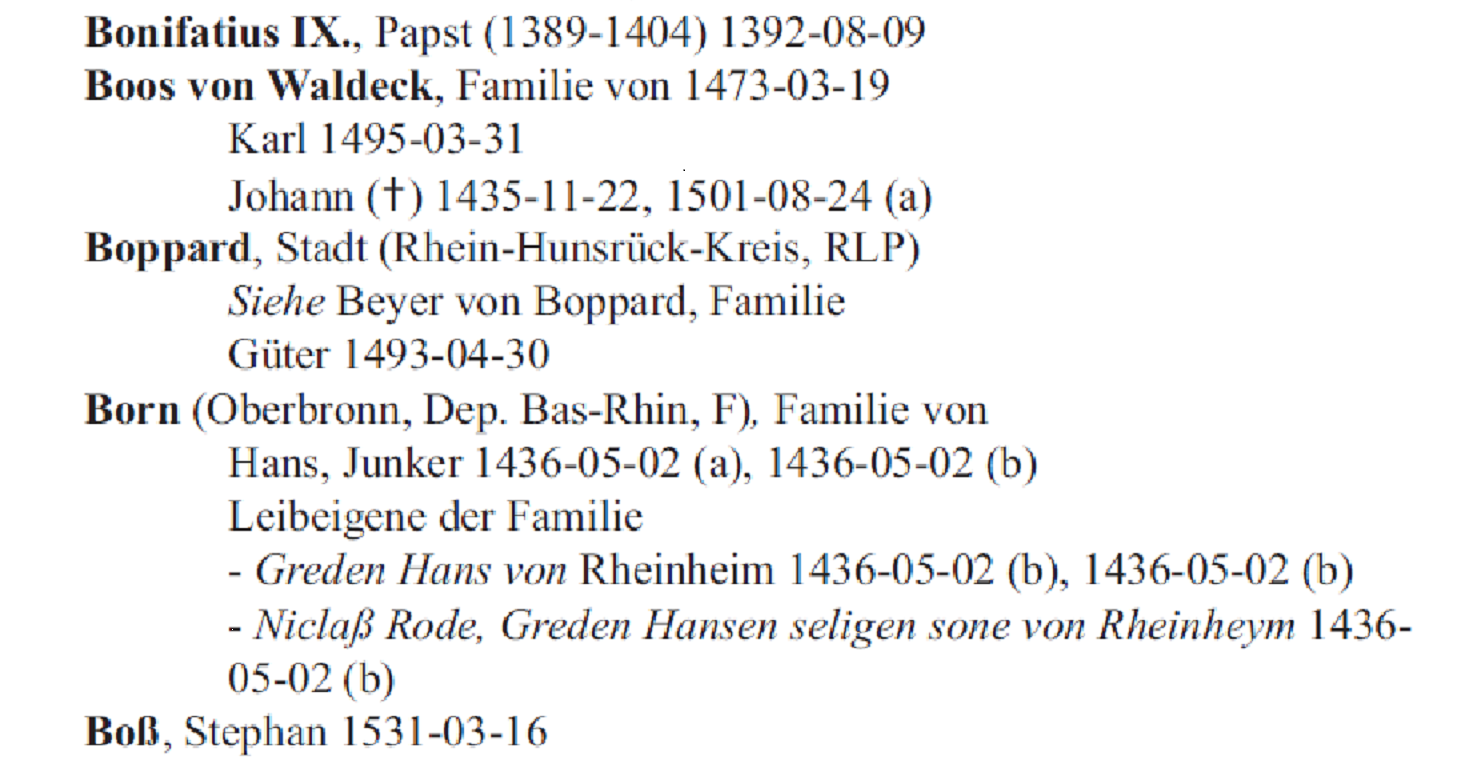
\includegraphics[scale=0.3]{img/index-examples}
  \caption{Examples for index entries taken from the Sbr-Regesten}
  \label{fig:index-examples}
\end{figure}
The index is a manually build list of entities that appear in the regests. It is the last part of the Sbr-Regesten and is 277 pages long. Figure~\ref{fig:index-examples} shows typical index entries taken from the Sbr-Regesten. The index entries differ from each other, but can roughly be divided into the following five groups: \textit{locations, landmarks, persons, families} and \textit{persongroups}. In total, there are 1035 index entries (see figure~\ref{fig:type-table} for the distribution of groups). 

\begin{figure}[h]
\centering
\begin{tabular}{|l|c|}
\hline
Type of index entry & Number of entries  \\
\hline
Location            & 550 \\
Landmark            & 22  \\
Person              & 103 \\
Persongroup         & 46  \\
Family              & 313 \\
Other               & 1   \\
\hline
sum         & 1035\\
\hline
\end{tabular} 
\caption{Distribution of index entries}
\label{fig:type-table}
\end{figure}

\subsection{Index Entries}
An index entry can intuitively be divided into two parts, which we name \textit{header} and \textit{body}. The header gives more details about the entity, e.g. where a location is located, what profession a person has or in which regest to find the entity. The body gives a list of concepts/entities which are in some (sometimes specified) relation to the index entity. For example \textit{Boos von Waldeck} (see figure~\ref{fig:index-examples}) would have the header \textit{Boos von Waldeck, Familie von 1473-03-19}. The remaining part of the index entry would be the body.

Irrespective of the group they belong to, index entries have some elements in common. Each index entry starts with its name, which is written in bold. The name might be followed by alternative or additional names. These are usually written in italics (which indicates that they are original text) and in parenthesis right after the name. The header of index entries usually ends with a set of numbers in the form of dates, which refer to the particular regests, where this entity is named. Right after these regest-references, there might appear references to other index entities. They start with the word \textit{siehe} (\textit{see}).

The body of an index entry is a list of concepts, which are related to the entity. For example \textit{Karl} stands in some relation to the family \textit{Boos von Waldeck}, namely he is a member of it. There exist different layers of such related concepts. If \textit{Karl} had a son for example, he could appear indented below \textit{Karl}. But apparently, a concept on the third level must not obligatorily be in relation with the one the first level. The house where Karl lived could appear below \textit{Karl} as well, although it is not directly related to the family. Often, the authors manually introduced a level between the index entity and the actual body-entities/concepts in order to group the items. For example \textit{Einwohner} or \textit{Güter}, below which there can be found a list of inhabitants/goods which in the regests appeared in relation with the index entity. Each concept might be followed by a set of numbers, which refers the reader to the regest in which the concept was named.

Apart from these commonalities, the headers and bodies are distinct for the different groups. The following sections describe the distinctive parts each of the five groups. 

\begin{figure}[h]
\centering
\begin{tabular}{|l|p{10cm}|}
\hline
\textbf{Group}        & \textbf{Possible types}  \\
\hline
location types & Dorf, Stadt, Stadtteil, Burgsiedlung, Burg,  ehem. Burg, Hofgut, Hof, Ort, Örtlichkeit, Gemeinde, Kloster,   Abtei, Schloss, Herrschaft, Herzogtum, Hzgt., Grafschaft,    Gft., Fürstentum, Kgr., Deutschordenskommende, Bistum,     Vogtei, Regierungssitz, Hochstift, Pfarrei, Erzstift, Erzbistum, Dekanat, Domstift, Reichsland, Deutschordensballei, Wasserburg, Mühle, Zisterzienserabtei, Region, Deutschordenshaus \\
\hline
landmark types & Berg, Gau, Talschaft, Bach, Tal, Landschaft, Au, Waldung, Wald, Gemeindewald \\
\hline
persongroups   & Notare, Grafen, Markgrafen, Herzöge, Bischöfe, Edelknechte, Herrn von, Herren, Fürsten, Personen, Könige, Ritter von, Einwohner, Päpste, Wildgrafen, Dominikaner \\
\hline
\end{tabular} 
\caption{Types for locations, landmarks and persongroups found in the index}
\label{fig:location-list}
\end{figure}

\paragraph{Locations}
The locations found in the index are geographical or political. They might also be buildings. Among them are towns, castles, parishes, kingdoms or mills. A full list of the types of locations found in the index can be found in figure~\ref{fig:location-list}. In the index entry, the type of location is usually specified right after the name or eventual additional names. It is often followed by district (Gemeinde, Stadt, Stadtverband, Kreis), region (Province, Bundesland or Departement) and/or country. Most of the locations are in Germany. The country is only specified, when the location is not in Germany. Sometimes additional descriptions of where to find the location can be found right after the type name (e.g. \textit{Dorf im Köllertal}, \textit{Hof bei St. Ingbert}). Locations also specify if a location is no longer inhabited. Entries of such abandoned villages (\textit{Wüstungen}) contain references where to find them in Staerk's catalogue\footnote{Dieter Staerk, Die Wüstungen des Saarlandes, Minerva-Verlag, Saarbrücken, 1974.}). %See figure~\ref{fig:location-example} for sample entries.

\begin{figure}[h]
  \centering
  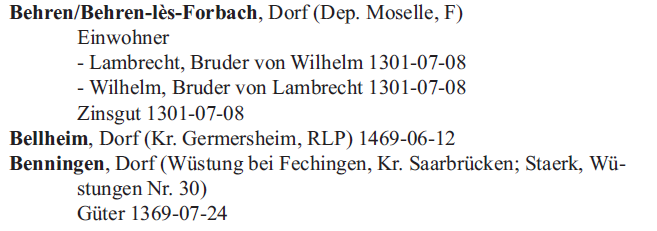
\includegraphics[scale=0.45]{img/location-example}
  \caption{Examples for location index entries taken from the Sbr-Regesten}
  \label{fig:location-example}
\end{figure}

\paragraph{Landmarks}
Landmarks (\textit{Flurnamen}) are geographical units as forests, mountains, valleys. For the whole list of landmarks found in the index, see figure~\ref{fig:location-list}. Landmarks do not provide any additional unique information.% See figure~\ref{fig:landmark-example} for sample entries.

\begin{figure}[h]
  \centering
  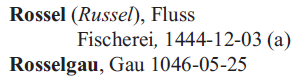
\includegraphics[scale=0.45]{img/landmark-example}
  \caption{Examples for landmark index entries taken from the Sbr-Regesten}
  \label{fig:landmark-example}
\end{figure}

\paragraph{Persons}
Person-headers may contain forenames, surnames, maiden names ans generational names (as \textit{Senior, the first, II.}). Additionally they can specify the role or occupation of the person, biographical information such as date of birth or date of the beginning the role and relations to other persons (e.g. \textit{married with, son of}).% See figure~\ref{fig:person-example} for sample entries.
\begin{figure}[h]
  \centering
  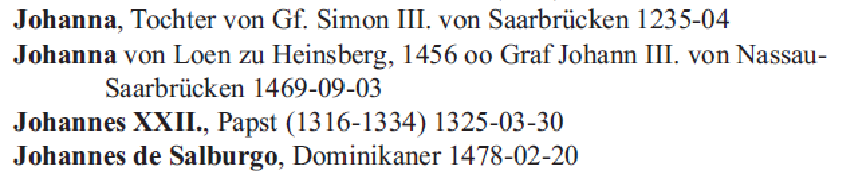
\includegraphics[scale=0.45]{img/person-example}
  \caption{Examples for person index entries taken from the Sbr-Regesten}
  \label{fig:person-example}
\end{figure}

\paragraph{Families}
Family-headers have no special elements. But their body can be defined more precisely. Family-bodies do not only represent a list of related entities/concepts, but they are a list of the members of the family. After each of them, the regest where it appeared might be specified. Below each family member (at the next level) there might appear concepts related to that specific member. This might again be a family member but not necessarily.
%%See figure~\ref{fig:family-example} for sample entries.

\begin{figure}[h]
  \centering
  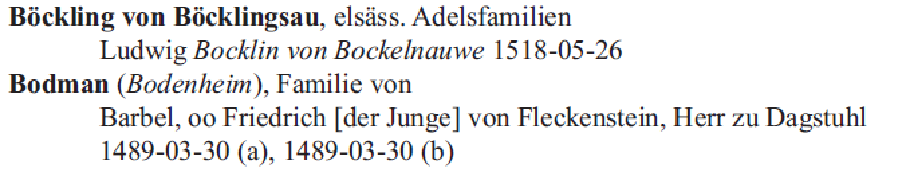
\includegraphics[scale=0.45]{img/family-example}
  \caption{Examples for family index entries taken from the Sbr-Regesten}
  \label{fig:family-example}
\end{figure}

\paragraph{Persongroups}
Persongroups are index entries that contain a group of persons. For example, there is a list for popes, for inhabitants of Saarbrücken, bishops etc. The complete list is shown in figure~\ref{fig:location-list}. The group name is specified in the header. Similar to the families, the header does not contain any specific elements, whereas the body is a list of concepts which can be specified more concretely. In the case of persongroups, each concept on the first level of the body is a person and member of the group. %See figure~\ref{fig:persongroup-example} for sample entries.

\begin{figure}[h]
  \centering
  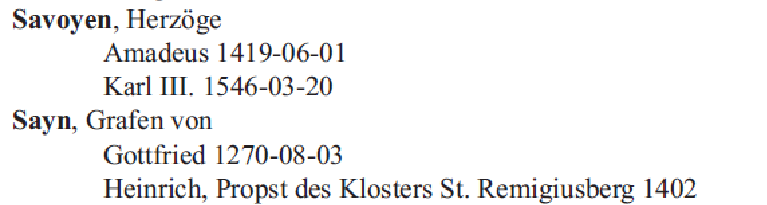
\includegraphics[scale=0.45]{img/persongroup-example}
  \caption{Examples for persongroup index entries taken from the Sbr-Regesten}
  \label{fig:persongroup-example}
\end{figure}

\paragraph{Others}
\label{sec:other-index-entry}
Only one index entry is very unusual and does not fit in any of the proposed groups. It is the entry \textit{Saarbrücken, Gliederung}, which shows an overview over the \textit{Saarbrücken} entry (see figure~\ref{fig:sb-gliederung}). The \textit{Saarbrücken} entry is the largest index entry with almost 100 pages. It is therefore split up into seven entries. \textit{Saarbrücken, Gliederung} gives an overview over these entries.

\begin{figure}[h]
  \centering
  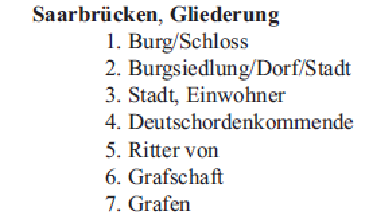
\includegraphics[scale=0.6]{img/sb-gliederung}
  \caption{The index entry \textit{Saarbrücken, Gliederung}}
  \label{fig:sb-gliederung}
\end{figure}


\subsection{XML Schema for the Index}

One of the main contributions of the Sbr-regesten project was to create an XML schema for the Sbr-regesten. The schema can be found in the file \texttt{sbr-regesten.xsd}.
It was as far as it was applicable designed to comply with the TEI Guidelines \footnote{TEI P5: Guidelines for Electronic Text Encoding and Interchange by the TEI Consortium, Version 2.0.2, 2012}.This section describes the schema for the index.

The index consists of an \texttt{index-info}, which contains general information about the index, followed by an unrestricted number of \texttt{items}. Each \texttt{item} represents an index entry and is either a location, a person, a landmark, a family or a persongroup. The schema covers each of the groups respectively.

Each index item requires the following attributes: 
\begin{itemize}
\item \texttt{id}: a unique id (e.g. item\_381)
\item \texttt{type}: location, landmark, person, family or persongroup
\item \texttt{value}: the name of the item (printed in bold in the printed Sbr-Regesten)
\end{itemize}

%%\begin{figure}[h]
%%\begin{verbatim}
%%<item id="item_661" type="persongroup" value="Notare">
%%\end{verbatim}
%%\label{fig:placeName}
%%\caption{\texttt{item} in TEI vs. \texttt{placeName} in the Sbr. Regesten schema.}
%%\end{figure}

An index \texttt{item} consists of an \texttt{item-header} and can also have an \texttt{item-body}. Both are abstract elements, which are substituted by the respective header and body types. This decision was made in order to have only one type of items with consecutive IDs, although the headers and bodies highly vary with depending on their type.


The header might for all header types end with the elements \texttt{mentioned-in}, followed by \texttt{index-refs}. \texttt{Mentioned-in} is of type \texttt{mentionings} and contains a sequence of references to the regests. The attribute \texttt{regest} specifies the id from the regest it refers to. \texttt{Index-refs} contains  a sequence of references to other index entries. The attribute \texttt{itemid} contains the id from the index item it refers to. texttt{Index-refs} are allowed to contain free text to insert key words/indications to make evident to the reader, that these are references to index entries (mostly \textit{siehe}).
The next sections will describe in more detail the elements, that items have depending on their type. They will also provide a marked-up example each header and body type.

\subsubsection{Headers}

\paragraph{Location-Header}
Figure~\ref{fig:location-header-xml} and \ref{fig:location-wuest-xml} show examples for location headers. Location headers contain the element \texttt{placeName}, which corresponds mostly to TEI's \texttt{placeName}. See figure~\ref{fig:placeName}for an example for a comparision between both. The Sbr-regesten schema adopts TEI's \texttt{settlement}, \texttt{district}, \texttt{region} and \texttt{country}. It introduces two new attributes for the settlement element, aside from \texttt{type}. It gets the additional attributes \texttt{abandoned-village} and \texttt{av-ref} to encode information about abandoned villages (\texttt{Wüstungen}). \texttt{Abandoned-village} denotes if the settlement is an abandoned village. In that case \texttt{av-ref} encodes the reference to the catalogue of Staerk \footnote{Dieter Staerk, Die Wüstungen des Saarlandes, Minerva-Verlag, Saarbrücken, 1974.}. Region types may be \texttt{Bundesland} (if located in Germany), \texttt{Departement} (in France) or \texttt{Province} (Belgium). \texttt{Country} has no attribute. TEI defines a \texttt{district} as “any kind of subdivision of a settlement, such as a parish, ward, or other administrative or geographic unit.”\footnote{TEI P5: Guidelines for Electronic Text Encoding and Interchange by the TEI Consortium, Version 2.0.2, 2012} In contrast, in our index-locations a \texttt{district} is any administrative unit below a \texttt{region} (Kreis, Gemeinde, Stadtverband).
Additional to the elements proposed by TEI, the index schema for locations has two more elements: \texttt{additional names} (which contains a list of additional names of the location) and \texttt{reference-point}, which contains further information not covered by\texttt{ district/region/country}. This information specifies where to find the location, e.g. \textit{Im Köllertal, bei St. Ingbert} (in the Köllertal, near St. Ingbert). All of the elements are optional (even settlement, as it also appears in the family headers, where \texttt{locations/placeNames} are given, without their names being explicitly specified.)   

\begin{figure}[H]
\centering
\begin{verbatim}
<location-header>
   <placeName>
      <settlement type="Dorf" w="false">Frauenberg</settlement>
      <addNames> (
         <addName>Frauwenberg</addName>)
      </addNames>, Dorf (
      <region type="Departement">Dep. Moselle</region>, 
      <country>F</country>) 
   </placeName>
   <mentioned-in>
      <reg-ref regest="regest_235">1452-12-26</reg-ref>, 
      <reg-ref regest="regest_984">1459-02-19</reg-ref>
   </mentioned-in> siehe 
   <index-refs>
      <index-ref itemid="item_534">Lenterdingen</index-ref>,
      <index-ref itemid="item_956"> Volkersweiler</index-ref>
   </index-refs>
</location-header>
\end{verbatim}
\label{fig:location-header-xml}
\caption{Sample \texttt{location-header} xml.}
\end{figure}

\begin{figure}[H]
\centering
\begin{verbatim}
<location-header>
   <placeName>
      <settlement type="Dorf" w="true" w-ref="Staerk, Wüstungen Nr. 19">
         Arschofen</settlement>
      <ddNames> (
         <addName>Arßhoffen</addName>)
      </addNames>, Dorf 
      <reference-point>im Köllertal</reference-point> (Wüstung, 
      <district>Gde. Gersweiler, Stadtverband Sb.</district>, 
      <region type="Bundesland">SL</region>; Staerk, Wüstungen Nr. 19) 
   </placeName>
</location-header>
\end{verbatim}
\label{fig:location-wuest-xml}
\caption{Sample \texttt{location-header} xml with \textit{Wüstung}.}
\end{figure}

\begin{figure}[H]
\centering
\begin{verbatim}
<placeName>
    <settlement type="city">Rochester</settlement>,
    <region type="state">New York</region>
</placeName>

<placeName>
    <settlement type="Stadt" w="false">Saarbrücken</settlement>,
    <region type="Bundesland">SL</region>
</placeName>
\end{verbatim}
\label{fig:placeName}
\caption{\texttt{placeName} in TEI vs. \texttt{placeName} in the sbr-regesten schema.}
\end{figure}


\paragraph{Landmark-Header}
Figure~\ref{fig:landmark-header-xml} shows an example for a \texttt{landmark-header}. Landmark-headers consist of the elements \texttt{geogName}, \texttt{mentioned-in} and \texttt{index-refs}. The element \texttt{geogName} is alluded to the TEI \texttt{geogName}, but contains exactly the two elements name and \texttt{addNames} (additional names).

\begin{figure}[H]
\centering
\begin{verbatim}
<landmark-header>
   <geogName type="Fluss">
      <name>Rossel </name>
         <addNames>(
         <addName>Russel</addName>)
      /addNames>
   </geogName>, Fluss 
</landmark-header>
\end{verbatim}
\label{fig:landmark-header-xml}
\caption{Sample for \texttt{landmark-header}.}
\end{figure}

\paragraph{Person-Header}
Figure~\ref{fig:person-header-xml} shows an example for a person-header. Person headers provide the element \texttt{person}. Person consists of \texttt{persName} and \texttt{description}, where \texttt{persName} is very close to TEI's \texttt{persName}. It contains (optional) \texttt{forename}, \texttt{surname}, \texttt{genName} (generational name, such as Senior, the first, II., etc., see TEI) and \texttt{roleName} (name of the role/occupation? of the person: Fürst, Herzog, Papst, official title/rank/position, see TEI). The only addition to TEI in \texttt{persName} is \texttt{maidenname} (maiden name). Also here we do not have a single additional name (\texttt{addName}), but the element \texttt{addNames}, which contains a list of \texttt{addName} elements. It is also important to know that a \texttt{person} has not only an item id (as the other headers do), but also an id that refers to the person itself. This is due to the fact, that the \texttt{person} element is also used in the \texttt{listing-body}. A person therefore has two attributes: \texttt{id} and \texttt{itemid}.
The other element of \texttt{person} is called \texttt{description}. It provides additional information about the person, such as occupation, relation to other persons (married to, son of, etc.). It is of type \texttt{content}, which means, that it can contain \texttt{quote} elements, if there is original text in the \texttt{description}.

\begin{figure}[H]
\centering
\begin{verbatim}
<person-header>
   <person id="person_412">
      <persName>
         <forename>Johann</forename> 
         <genName>I.</genName>, 
         <roleName>Graf</roleName>
      </persName>
     <description> von Saarbrücken-Commercy (1307-1341), 
                    oo Mathilde von Apremont    </description>
   </person>
   <mentioned-in>
      <reg-ref regest="regest_543">1310</reg-ref>, 
      <reg-ref regest="regest_1353">1310-10-21</reg-ref>, 
   </mentioned-in>
</person-header>
\end{verbatim}
\label{fig:person-header-xml}
\caption{Sample for \texttt{person-header}.}
\end{figure}

\paragraph{Family-Header}
Figure~\ref{fig:family-header-xml} shows an example for a \texttt{family-header}. Family headers consist of the elements \texttt{family-name}, \texttt{location}, \texttt{mentioned-in} and \texttt{index-refs}. \texttt{Family-name} consists of name and \texttt{addNames} (additional names). \texttt{Location} is of type \texttt{placeName}, which is the same type that \texttt{location-header}s have. See section \textit{location-header} for more details.

\begin{figure}[H]
\centering
\begin{verbatim}
<family-header>
  <family-name>
     <name>Brandscheid</name>
     <addNames>
        <addName>Brandscheidt<addName>       
     </addNames>
  </family-name> (
  <location>
     <district>Kr. Bitburg-Prüm</district>, 
     <region type="Bundesland">RLP</region>
  </location>), Familie von 
</family-header>
\end{verbatim}
\label{fig:family-header-xml}
\caption{Sample for \texttt{family-header}.}
\end{figure}

\paragraph{Persongroup-Header}
Figure~\ref{fig:persongroup-header-xml} shows an example for a \texttt{persongroup-header}. Persongroup headers consist of the elements \texttt{group-name}, \texttt{mentioned-in} and \texttt{index-refs}. \texttt{Group-name} is a string, containing the name of the persongroup.
not TEI's \texttt{listperson}, because it would be the actual list, which in our case is in the body..

\begin{figure}[H]
\centering
\begin{verbatim}
<persongroup-header>
   <group-name>Notare </group-name>
</persongroup-header>
\end{verbatim}
\label{fig:persongroup-header-xml}
\caption{Sample for \texttt{persongroup-header}.}
\end{figure}

\subsubsection{Bodies}
There are two different types of bodies: \texttt{Concept-body} and \texttt{listing-body}.

\paragraph{Concept-body}
TODO: A concept-body contains related concepts. Each related concept consists of at least one concept or person (either only concepts or only persons)
concept:
name
description
mentioned-in
related-concepts
person
see person-header-person
We might also find other concepts in relation to the first lever member.
\begin{figure}[H]
\centering
\begin{verbatim}
<concept-body>
   <related-concepts>
      <concept>
         <name> Einwohner </name>
         <related-concepts> -
            <concept>
               <name> Hans gen. Phennewert </name>
               <mentioned-in>
                  <reg-ref regest="regest_64">1455-11-24</reg-ref>
               </mentioned-in>
            </concept> -
            <concept>
               <name> Philipps Pfenwert von Hermanßhusen</name>
               <description>, Bürger zu Saarbrücken, oo Ursulla </description>
               <mentioned-in>
                  <reg-ref regest="regest_756">1510-11-09</reg-ref>, 
                  <reg-ref regest="regest_834">1521-12-24</reg-ref>
               </mentioned-in>
            </concept>
         </related-concepts>
      </concept>
      <concept>
         <name> Güter </name>
         <mentioned-in>
            <reg-ref regest="regest_43">1296-12-29</reg-ref>
         </mentioned-in>
      </concept>
   </related-concepts>
</concept-body>
\end{verbatim}
\label{fig:concept-body-xml}
\caption{Sample for \textit{concept-body}.}
\end{figure}

\paragraph{Listing-body}
Figure~\ref{fig:listing-body-xml} shows an example for a \texttt{listing-body}. A listing-body consist of the element \texttt{members}. \texttt{Members} consists of a list of persons (same type as the persons appearing in a person-header). Each person can have related concepts, which recursively can have related concepts again, as in a concept-body.
That means, that in a \texttt{persongroup} or \texttt{family}, the first layer displays members of that family or group. The concepts on the levels beyond might also be family or group members but not obligatory. Therefore they are not modelled as members on their own, but as related-concepts of that member.

\begin{figure}[H]
\centering
\begin{verbatim}
<listing-body>
  <members>
     <person id="person_89">
        <persName>
           <forename> Dietrich </forename>gen.
           <addNames>
              <addName> Gebürghin </addName>
           </addNames>
        </persName>
        <mentioned-in>
           <reg-ref regest="regest_823">1460-12-01</reg-ref>
        </mentioned-in>
        <related-concepts> -
           <concept>
              <name> Knecht Peter </name>
              <mentioned-in>
                 <reg-ref regest="regest_823">1460-12-01</reg-ref>
              </mentioned-in>
           </concept>
        </related-concepts>
     </person>
     <person id="person_90">
        <persName>
           <forename> Jakob von Brandscheid</forename>
        </persName>
        <description>, Amtmann zu Saargemünd </description>
        <mentioned-in>

           <reg-ref regest="regest_934">1519-03-23</reg-ref>
        </mentioned-in>
     </person>
  </members>
</listing-body>
\end{verbatim}
\label{fig:listing-body-xml}
\caption{Sample for \texttt{listing-body}.}
\end{figure}


\subsection{Index Extraction}
In order to convert the Sbr-Regesten into an XML, relevant pieces of information have to be extracted from the HTML and tagged according to the schema. Additionally, the regests and index entries are written into the database \texttt{sbr-regesten.db}.


\begin{figure}[h]
  \centering
  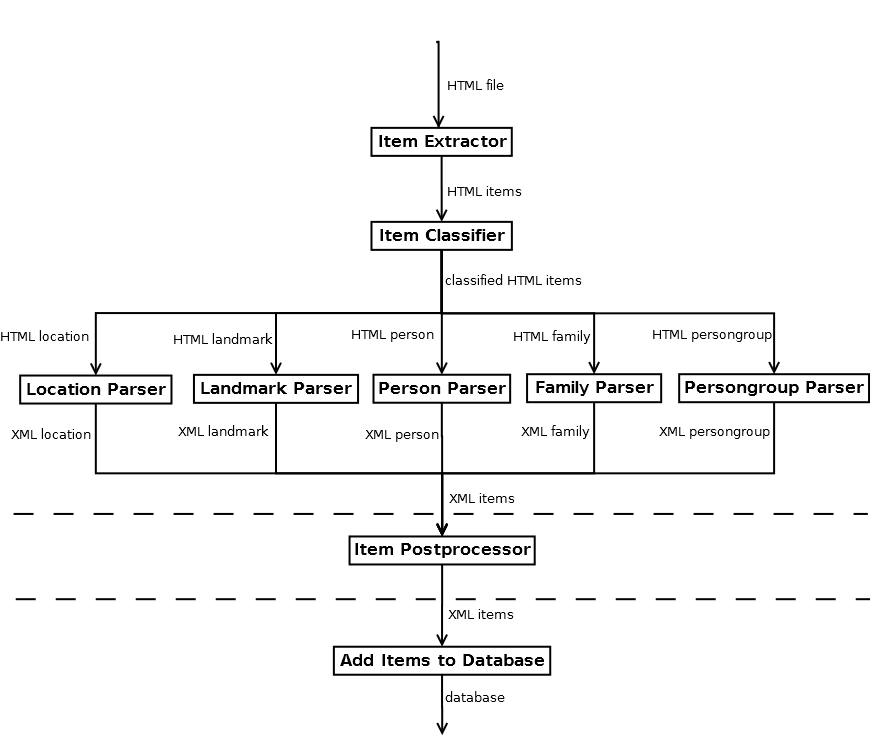
\includegraphics[scale=0.5]{img/index-extractor}
  \caption{Simplified architecture of \texttt{index\_extractor.py}.}
  \label{fig:index-extractor}
\end{figure}

This chapter will describe in more detail how the XML for the index is extracted. 
Figure~\ref{fig:index-extractor} shows the basic architecture of the process of index extraction (\texttt{index\_extractor}). Note it does not display any classes, but is aimed to illustrate the logical structure/workflow of the index\_extractor to demonstrate its functionality. In short, the \texttt{index\_extractor} module finds the index in the HTML and extracts single index items. These are later postprocessed, before yielding the final XML for the index entries and writing them form the XML file into the database.

The index\_extractor is divided into three modules (to be found in \texttt{extraction/index\_utils}):

\begin{itemize}
\item index\_to\_xml converts the HTML to an almost complete XML
\item index\_xml\_postprocess postprocesses the XML, solving the references to the index entries
\item index\_to\_db extracts the index-items from the XML and writes them into the database
\end{itemize}

The separation of converting the index into XML and writing them into the database, has two reasons: it is easier structured and it is possible to manually correct the XML-file before adding the items into the database.

\subsubsection{From the Index to the XML}
The module \texttt{index\_to\_xml.py} uses the python package BeautifulSoup to process the HTML and convert it into XML. One problem that arose was that due to the maximum recursion limit the very deep structured index entry \textit{Saarbrücken, Burgsiedlung/Dorf/Stadt} could not be processed. Therefore the recursion limit had to be increased\footnote{This seems to be a common problem, when using BeautifulSoup. See \href{http://blog.pablohoffman.com/maximum-recursion-limit-in-python}{this blog-entry on maximum-recursion-limit-in-python}.}.

Figure~\ref{fig:index-to-xml} shows the call graph of the basic functions of \texttt{index\_to\_xml.py} (excluding the preprocessing steps and the solving of index entries form the "siehe" list).

\begin{figure}[h]
  \centering
  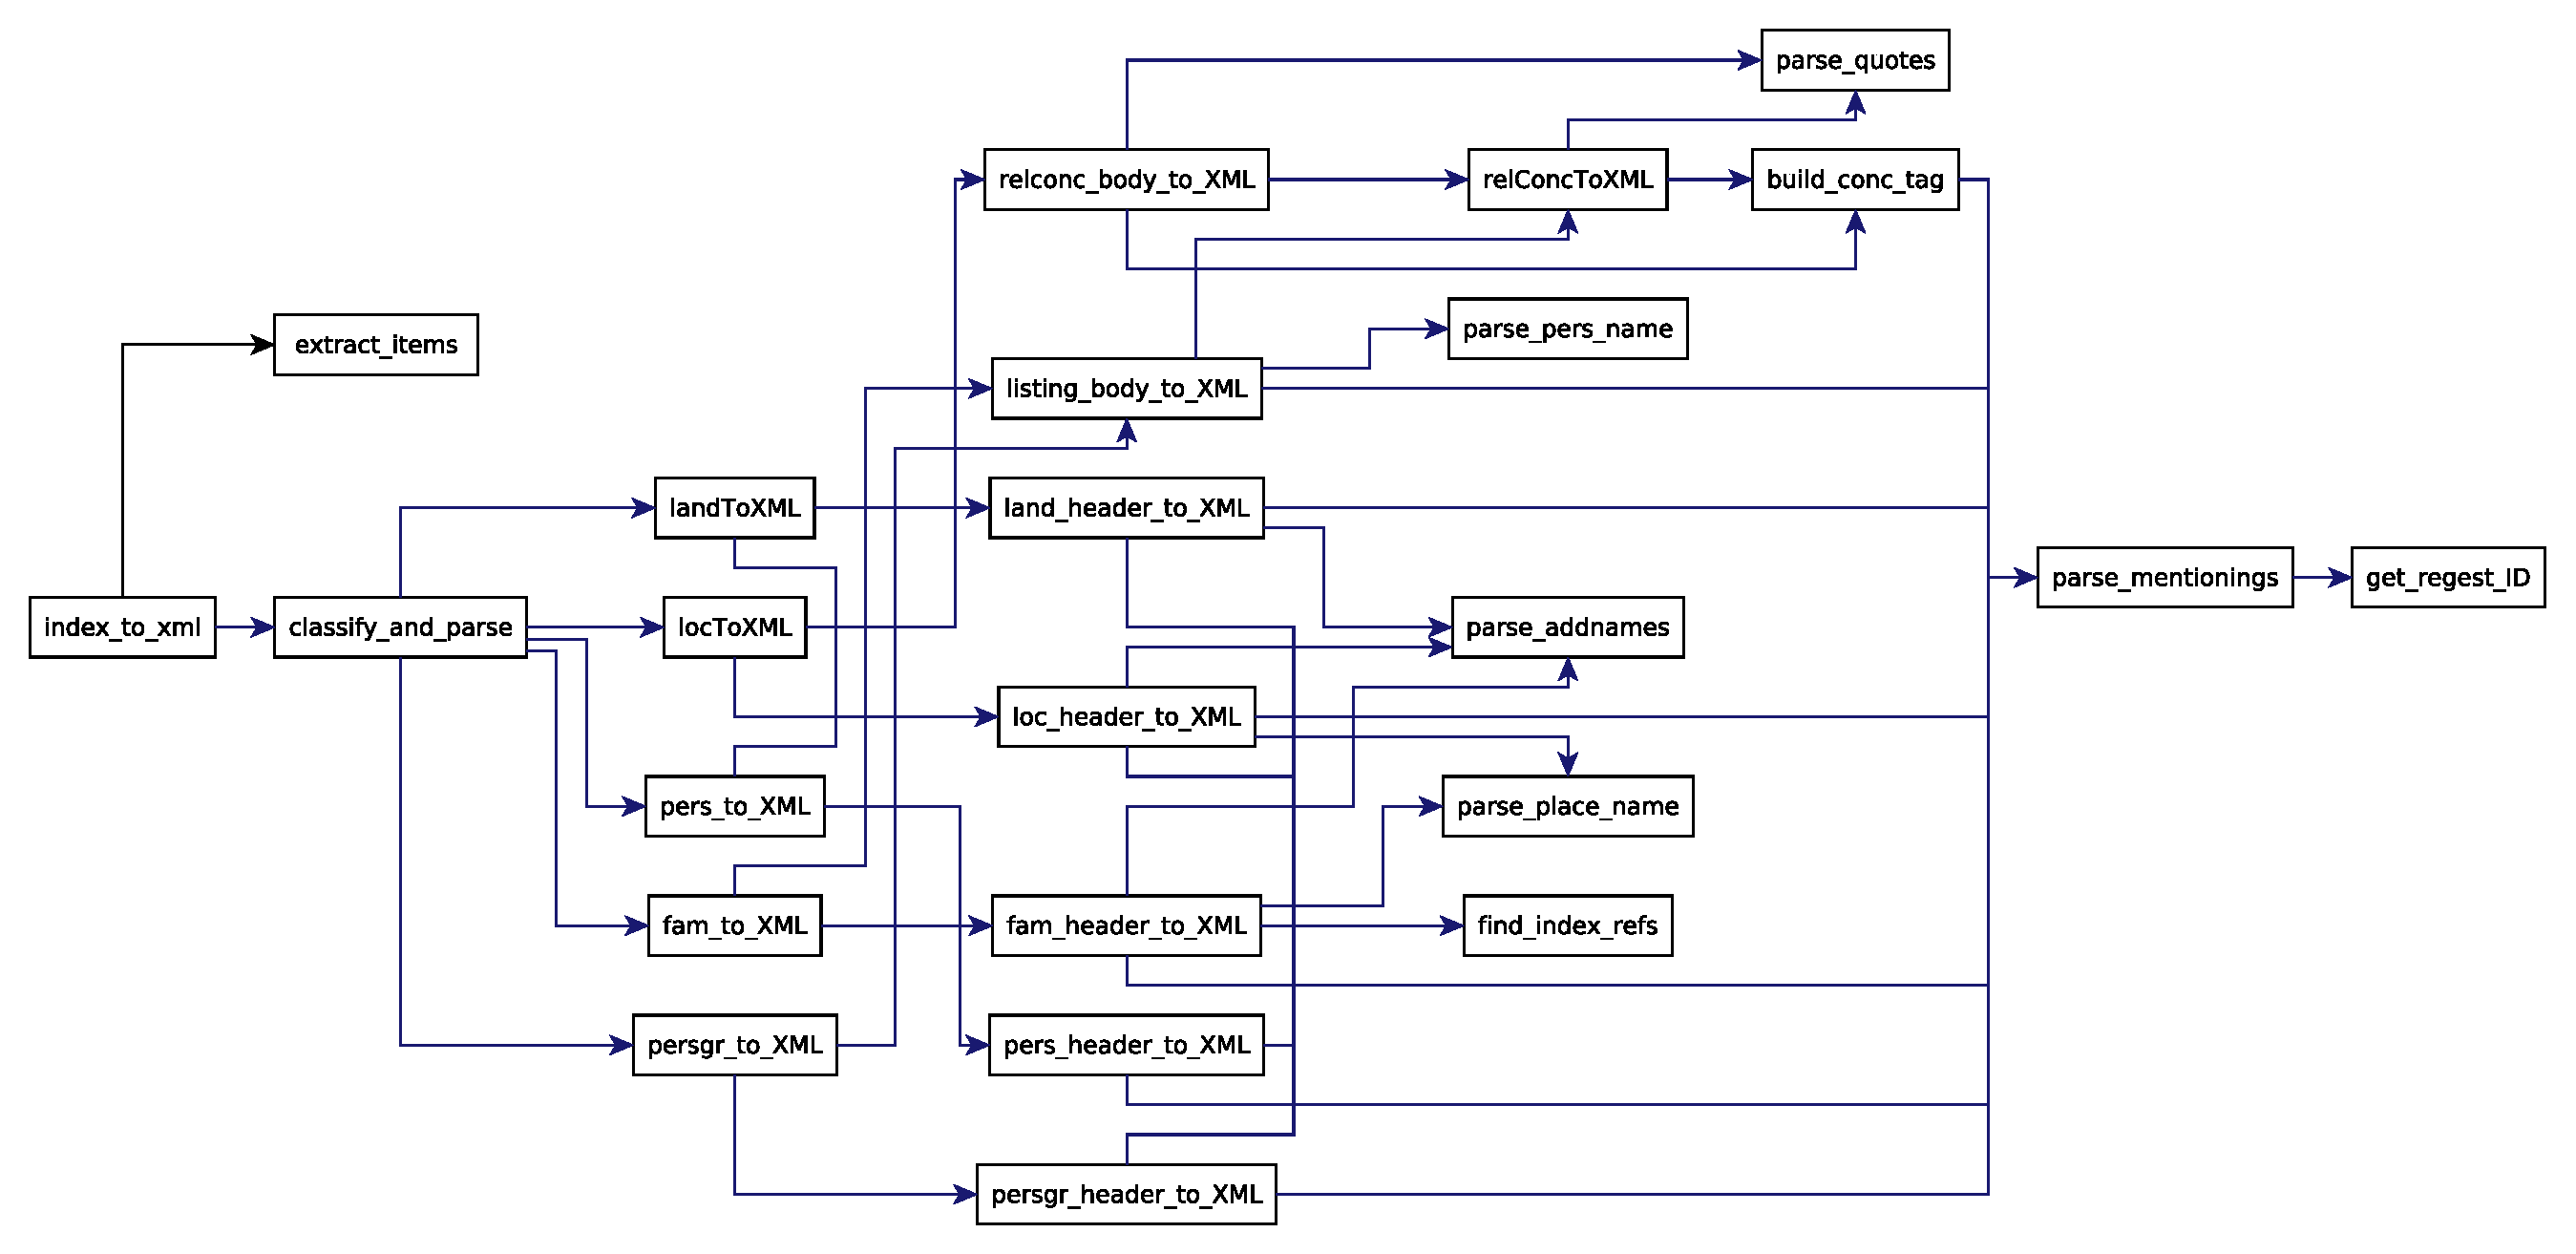
\includegraphics[scale=0.35]{img/index-to-xml}
  \caption{Basic call graph of \texttt{index\_to\_xml}}.
  \label{fig:index-to-xml}
\end{figure}

\paragraph{ItemExtractor}
The ItemExtractor (function \texttt{extract\_items()}) reads the HTML source and converts it into a BeautifulSoup instance. The extraction of the single index items is very straightforward, as the HTML provides tags for paragraphs (\texttt{<p>}). Each index item is a paragraph. In order to find the beginning of the index, the paragraph starting with the keyword \textit{Index} is searched. Once it is found, the ItemExtractor tags the next non-empty paragraph as \texttt{<index-info>}. Each of the following non-empty paragraphs is recognized as index-item. It obtains an id and is preprocessed (irrelevant tags are deleted from the HTML and some irregularities are overcome). An instance of Index Item is created, which divides the HTML-paragraph into a header and body field. The ItemExtractor finishes processing the paragraphs when reading more than 10 empty paragraphs in a row. In that case we assume the index-section to be finished. It can not be solved via a key as for the beginning of the index or as in the extraction of the other parts of the books as the index is the last part of the book, only followed by the footnotes (in the HTML file). All extracted item objects are stored in a list and are in the next step given to the ItemClassifier.

\paragraph{ItemClassifier}
The ItemClassifier is implemented by the function \texttt{classify\_and\_parse}. It classifies the items and forwards them to the corresponding parsers, where they are parsed and returned. The ItemClassifier obtains the list of item objects and searches the header of each item for a set of names/keys (retrieved by bootstrapping, see figure~\ref{fig:regex} \footnote{Note, that the order of the keys and the matches are relevant, as some are more confident than others.}). In this way it decides for each item whether it belongs to the group \textit{location, landmark, person, family, persongroup} or \textit{siehe}. It forwards the item to the corresponding parser (\texttt{loc\_to\_XML(), land\_to\_XML, pers\_to\_XML, fam\_to\_XML} and \texttt{persgr\_to\_XML} respectively). The items stored in the \textit{siehe} list contain no direct information about the group they belong to. But they contain references to other index entries. Assuming that referring and referenced entry have the same type, they are forwarded to the corresponding parser after having solved the reference. Items that do not contain any of the keywords are stored in the list \textit{unclassified} and are not further processed. This is the case for the entry \textit{Saarbrücken, Gliederung} as this is a rather unusual entry (see~\ref{sec:other-index-entry}).

\begin{figure}
\centering
\begin{verbatim}
famMatch = re.search('[Ff]amilie|Adelsgeschlecht', header)

locMatch = re.search('[Ss]tadt,|Stadtteil|Dorf|Burg |Hof |Hofgut|'\
                     'Gemeinde |Ort |.rtlichkeit |Kloster|Schloss|'\
                     'Herrschaft|Gft\.|Kgr\.|Region|Gebiet|Abtei|'\
                     'Land |Kgr\.|Herzogtum|Hzgt\.|[Gg]rafschaft|'\
                     'F.rstentum|Deutschordenskommende|RLP|Gde\.|'\
                     'Bistum|Vogtei|Regierungssitz|Hochstift|'\
                     'Pfarrei|W.stung|F\)|Erzstift|, Erzbistum|'\
                     'Dekanat|Domstift|Reichsland|Deutschordensballei'\
                     '|M.hle|Wallfahrt|Land |Reise|lothr. Amt|'\
                     'Deutschordenshaus|[Ss]tadt (?!S)', header)

grpMatch = re.search('Notare|, Grafen|, Markgrafen|[Hh]erz.ge|'\
                     '[Bb]isch.fe|Edelknechte|Herrn von|[Ff].rsten|'\
                     'Personen|K.nige|Ritter von|Einwohner|P.pste|'\
                     'Wildgrafen|Herren|(?<!, )Dominikaner', header)

persMatch = re.search('Bischof|Pastor|Graf |Papst |II\.|I\.|III\.|'\
                      'IV\.|V\.|Hzg\.|Bf\.|Adliger|Herr |Frau |Kg\.|'\
                      'Elekt|meister|Ritter|, Schulthei.|, Herzogin|'\
                      'Amtmann|Lehensmann|Vetter von|Markgraf |'\
                      'Pfalzgraf|Ebf\.|, Herzog|, Dominikaner|Hans|'\
                      'Erzpriester|[dD]iakon|Provinzial|r.m\. K.nig|'\
                      'Kammermajor|Witwe|Junker|Stephan|Jacob|Klaus|'\
                      'Elisabeth|Fabricio|Nikolaus|Alheim|Gerbod', \
                      header)

landMatch = re.search('Fluss|Berg|gau[ ,]|Gau|Bach|Tal|Landschaft|'\
                      'Wald|Waldung|Gemeindewald|Au|furt|Engenberg', \
                      header)

\end{verbatim}
\label{fig:regex}
\caption{xxx.}
\end{figure}


\paragraph{ItemParser}
Once the item is classified it is passed to its corresponding ItemParser. There is an item parser for each of the five groups. It forwards the header to the specific header parser of its group and the body to one of the two body parsers. It then adds the parsed item to an itemList.
Each of the headerParsers returns also the name of its entry. This is taken as \texttt{value} for the items. \texttt{id} TODO

E.g. the location paser passes the location header to the locationHeaderParser, which returns an XML location-header and the name of the item. This one is taken as value attribute. The id obtained by the ItemExtractor is taken as id attribute and the type is added. In the case of location, location. The other four parsers proceed analogously.

\paragraph{Location-Header-Parser}
The parser for the location headers (\texttt{loc\_header\_to\_XML}) builds a \texttt{<location-header>}, placeName and settlement. The latter gets the attributes \texttt{abandoned-village} and \texttt{av-ref} It looks for the keyword \textit{W.stung} to decide whether it is an abandoned village and sets abandoned village to true/false. The regular expression \texttt{Staerk, W.stungen Nr. [0-9]{1,2}} is extracted and taken as value for \texttt{av-ref}. The name of the settlement (added to the settlement tag) is extracted from the HTML via the \texttt{<b>} tag. From the rest of the HTML, the additional names are parsed, exploiting existing parenthesis and \texttt{<i>} tags. From the rest of the HTML location-header, all HTML tags are deleted before the rest is processed. Then references to the regests and to other index entries are parsed by the respective parsing functions (see section~\ref{sec:reg-refs} and \ref{sec:index-refs}). The remaining string is searched for the type of the settlement (for the whole list see figure~\ref{location-list}). If one of the keywords is found it is taken as value for the attribute \texttt{type} of \texttt{settlement}. The rest of the string is parsed by the function \texttt{parse\_place\_name} (see section~\ref{sec:addNames}). Afterwards, the placeNameTag is added to the location-header, as well as the references to the regests and the references to the index. The header is now parsed.

\paragraph{Landmark-Header-Parser}
The Landmark-Header-Parser is implemented by the function \texttt{land\_to\_XML}. It builds a BeautifulSoup item \texttt{<landmark-header>} and adds a \texttt{<geogName>} tag to it. The landmark's name is extracted via the \texttt{<b>} tags in the HTML and added to a \texttt{<name>} tag, which is appended to the \texttt{geogName}. The remaining HTML is passed to the AddNameParser in order to extract additional names, possibly appearing in the beginning. The remaining part is flattened to a string, whose end is searched for index-refs and mentionings. The remaining middle part is thereafter searched for a set of keys for the type of landmark. See figure~\ref{fig:location-list}. If none of the keys is found in the rest string, the name of the landmark is searched. This is because the type is often not explicitly specified if it is already contained in the name, e.g. \textit{Dirminger Tal, Ensdorfer Au}.

\paragraph{Person-Header-Parser}
The person headers are parsed by the function \texttt{pers\_header\_to\_XML()}. It builds a \texttt{<person-header>} BeautifulSoup Tag and adds a \texttt{<person>} tag to it. The latter obtains a continious id with the pattern \texttt{person\_[0-9]+}. A tag \texttt{<persName>} is added to the \texttt{person}. The \texttt{name} is extracted exploiting the \texttt{<b>} tags of the HTML. Thereafter, the HTML tags are aborted and index-refs and mentionings are extracted from the end of the remaining string(see section~\ref{sec:index-refs} and \ref{sec:reg-refs}). The remaining middle part is then used to extract \texttt{forename, surname, genName and roleName}. A set of keywords (e.g. \textit{der Dritte, der Junge, Jr} for \texttt{genName} and \textit{Kaiser, Herzogin, Graf} for \texttt{roleName}). A list of forenames is provided by the file \texttt{resources/forenames.txt} which is imported at the beginning of \texttt{index\_to\_xml.py} and augmented during the extraction by the Listing-Body-Parser. A set of regular expressions describes possible combinations of these different names. The first matching rule is chosen and the item header tagged accordingly. The remaining part of the string is tagged as \texttt{<description>}. At the end the extracted index-refs and mentionings are added to the \texttt{<person-header>} tag.

\paragraph{Family-Header-Parser}
The headers of family items are parsed by the function \texttt{fam\_header\_to\_XML}. A \texttt{<family-header>} tag is created and a tag \texttt{<family-name>} is appended to it. The latter contains the name of the family extracted from the HTML via the \texttt{<b>} tags. Afterwards, the \texttt{<b>} tag is deleted and the rest of the HTML is searched for additional names. The rest of the HTML that does not contain any additional names is converting into a tag-less string. If this contains an opening parenthesis before the next word, the content of these parenthesis are detected to be a location, which is parsed by the placeName Parser (see section~\ref{sec:addNames}), which also parses the corresponding part from the location headers. The part following the parenthesis (if there were such, elsewise, the whole remaining string) is searched for index-refs and mentionings.

\paragraph{Persongroup-Header-Parser}
The Parser for persongroup-headers is the least complex headerParser, due to the simplicity of the actual headers and the XML schema. A \texttt{<persongroup-header>} tag is created. The HTML-tags are deleted and index-refs and mentionings are found at the end of the string. The remaining part is tagged as \texttt{<group-name>}. \texttt{group-name, index-refs} and \texttt{mentionings} are added to \texttt{persongroup-header}.

\paragraph{References to the index}
\label{sec:index-refs}
References to the index can be found at the very and of an index entry (regardless its type). They start with the keywords \textit{siehe} or \textit{siehe auch}, e.g. \textit{siehe Lenterdingen, Volkersweiler}. The function \texttt{find\_index\_refs} therefore recognizes strings starting with one of these keyword and ending with the end of the string as index-refs. As the references can not be solved at the time of extracting the index (references can refer to future index entries), they are not further processed, but only tagged with \texttt{<index-refs>}. The further division into the single index references and their solving does not take place until the post-processing step (see section~\ref{sec:postproc}).

\paragraph{References to the regests}
\label{sec:reg-refs}
The references to the regests are given by the date of the regest, e.g. \textit{1377-03-08 (nach), 1065-04-03, 1277-07-02 (b)}. The are not exactly the same as the titles of the regests. They usually contain only the date plus the information that is crucial for disambiguation. But this does not seem to be very consistent. They may occur at the end of \texttt{related-concepts}, and at the end of each type of index-header, only possibly followed by references to the index (index-refs).
The function \texttt{parse\_mentionings} recognizes the references to the regests in a given string (by using a regular expression). It builds a \texttt{<mentioned-in>} tag. It starts form the end of the string and tries to find one reference after the other. It tags it as \texttt{<reg-ref>} and adds as attribute \texttt{regest} the id of the regest it refers to. This part is carried out by the function \texttt{get\_regest\_ID}. Once, the precedent part was not recognized as reference, \texttt{parse\_mentionings} finishes.


\paragraph{Parsing of additional names \texttt{(parse\_addnames)}}
\label{sec:addNames}
\texttt{parse\_addnames} obtains a flat HTML element and extracts additional names. Additional names are written in italics and in parenthesis. Therefore the parser looks for \texttt{<i>} tags surrounded by parenthesis. The string inside contains the additional names, which are separated by commas. Each is tagged with \texttt{<addName>} and added to a \texttt{<addNames>} tag.

\paragraph{Concept-Body-Parser}

\paragraph{Listing-Body-Parser}


\paragraph{Postprocessing}
\label{sec:postproc}
\texttt{index\_xml\_postprocess.py} takes the temporary file \texttt{index.xml} as input, which was produced by \texttt{index\_to\_xml.py} and deletes it after it is used. It looks for all references to index entries and tries to solve them, now that the whole index is already parsed. It replaces the corresponding parts and then adds the parsed index to \texttt{sbr-regesten.xml}.

\subsubsection{From the Index XML to the Database}
\texttt{index\_to\_db.py} takes the \texttt{sbr-regesten.xml} as input and processes the index items. It creates an entry in the database, extracts the tags from the item and adds the information to the fields defined in the model (see section~\ref{sec:data-model}).





\subsubsection{Future Work}

This section presents possible next steps for expanding the index schema, the index extraction and possible further uses. Depending on the use or queries of the Sbr-regesten, different expansions will have priority. In order to manipulate the regesten, a copy of the source code is requiered. To obtain such, see section~\ref{sec:git}.
\paragraph{References to the Regests}
At the time of developing the index extraction, the regest part of the book was not extracted or written into the database yet. Once this is the case, the first expansion of the current code would be to solve the references to the regests. The references are already recognised and tagged with reg-ref. Each reg-ref is supposed to store the id of the regest it refers to in the attribute regest. At the moment, this is not yet the case. The function \texttt{get\_regest\_ID} in \texttt{index\_to\_xml.py} returns the correct id only in cases where the date in the form "1532-11-24" is sufficient to disambiguate the regests. In other cases it returns the dummy id regest\_99999. We would recommand to reimplement the function \texttt{get\_regest\_ID} and solve the references directly searching the database, as the regests are added to the database before \texttt{index\_to\_xml.py} is called. To include the references also in the database, the function \texttt{ment\_to\_db} in \texttt{index\_to\_db.py} has to be implemented.

\paragraph{Extracting Person Names}
TODO: The index extractor allows the user to provide a list of forenames (\texttt{resources/forenames.txt}. During the extraction of the index it uses the list to recognize forenames and expands it at the same time. ...
list of forenames as input, postprocess similar to siehe, manually increment list with forenames from other sources. Same would be possible for surnames

\paragraph{Semantic Network}
The regests and the index do not provide only information about entities, but also about the relations they have. This becomes evident especially in the case of persons. The index already provides information such as "married with" or "son of". This information could be extracted to build networks of relations between persons.

\paragraph{Quotes}
The HTML provides information about which parts of the text are original text. Such sections are marked with italics (<i>). To mark original text the Sbr-regesten schema introduces the element 'Quotes'. This is mainly used in the regests. In the index quotes are only possible in the description part of the bodies. The tag <addNames> implicitly encodes this information as they extract text in italics. Otherwise this information gets lost during the process of extraction. But we can imagine the usefulness of conserving information about original text also in other parts of the index, we propose to expand the schema to allow quotes.

\paragraph{Expand References to the Index}
TODO: References to the index are only found and solved if they appear in the header right after the mentionings. But in some cases such references occur in other places as well (often in the bodies or before the district). The schema could be adapted to allow \texttt{reg-refs} there as well. They would have to be marked by texttt{index\_to\_xml.py} and would then (automatically) be extracted by the existing the \texttt{parse\_siehe} function in \texttt{index\_xml\_postprocess}.